One goal of the {\sc Cleo III} resonance program is to measure
$\Gamma_{ee}$ (leptonic decay width) of $\Upsilon(1S)$,
$\Upsilon(2S)$, and $\Upsilon(3S)$ to high precision ($\sim$2\%).

This measurement takes advantage of a relation between $\Gamma_{ee}$
and the total hadronic yield of each resonance:
\[\Gamma_{ee} = \Gamma(\Upsilon \to e^+ e^-) =
    \frac{\mbox{$M_\Upsilon$}^2}{6 \pi^2}
    \frac{\Gamma_{\mbox{\small total}}}{\Gamma_{\mbox{\small hadrons}}} \int d\mbox{\sc \small Energy \,
    \sigma(e^+ e^- \to \Upsilon \to \mbox{\small hadrons.})}
\]
The energy of the $e^+e^-$ center of mass system was scanned over each
of the $\Upsilon$ resonance masses, giving peaks in hadronic
cross-section versus energy.  These were fit to obtain total yields,
from which $\Gamma_{ee}$ is calculated.  For the $\Upsilon(1S)$,
$\Upsilon(2S)$, and $\Upsilon(3S)$ respectively, 0.13 fb$^{-1}$, 0.10
fb$^{-1}$, and 0.10 fb$^{-1}$ was collected to scan each resonance
peak, along with 0.23 fb$^{-1}$, 0.28 fb$^{-1}$, and 0.10 fb$^{-1}$,
for continuum subtraction and about 1 fb$^{-1}$ at the points of
maximum hadronic cross-section.

\begin{figure}[p]
  \begin{center}
    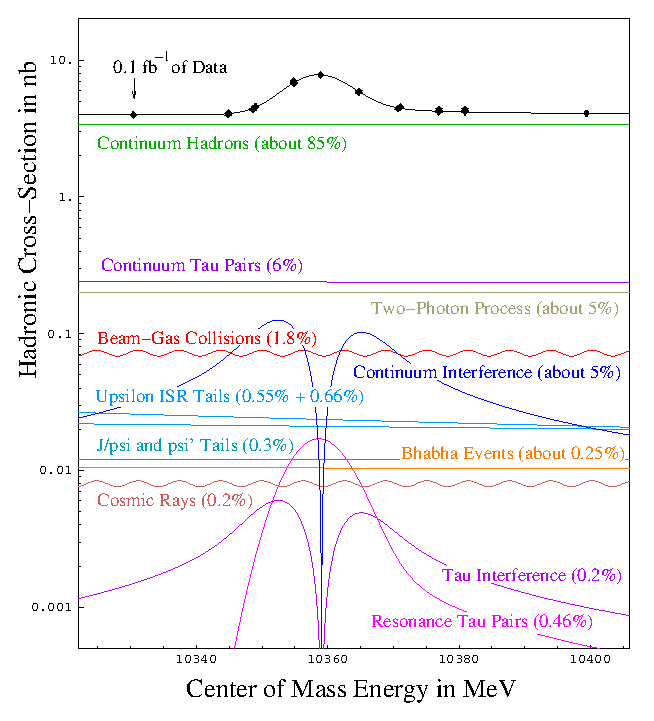
\includegraphics[width=0.9\linewidth]{pivarski1.eps}
  \end{center}
  \label{Gammaeebck}
\end{figure}

Figure \ref{Gammaeebck} shows the primary
backgrounds to $e^+ e^- \to \Upsilon(3S) \to \mbox{hadrons}$.  These
backgrounds have minimal effect on the shape of the peak (and
therefore $\Gamma_{ee}$) because they are either flat or very small.
The most significant three are $\Upsilon$ production with
initial-state radiation (which has a 0.1\% theoretical uncertainty,
from the calculation of Kureav and Fadin\cite{kureavfadin}), extra
events due to beam-gas interactions (which were carefully cut and
estimated using single-beam tests), and from the continuum-resonance
interference term of $e^+e^- \to q\bar{q}$ (which was calculated and
included in the shape function).

The total uncertainty in this measurement of $\Gamma_{ee}$ will be
dominated by systematic errors in energy measurement stability,
acceptance, integrated luminosity, and backgrounds, though only the
uncertainties due to the backgrounds have been studied in detail.
Figure \ref{Gammaeebck2} is a table of the
uncertainty in $\Gamma_{ee}$ for each resonance due to uncertainties
in handling a given background.  The total uncertainty due to
backgrounds is 0.1\% -- 0.2\% (the final row in the table), which is
comparable to the statistical uncertainties of 0.1\%, 0.3\% and 0.5\%
for $\Upsilon(1S)$, $\Upsilon(2S)$, and $\Upsilon(3S)$, respectively.

\begin{figure}[hbt]
  \large
  \begin{minipage}{\linewidth}
    \begin{tabular}{p{4.5cm} c c c}
      \mbox{\Large Contribution to Uncertainty in yield (and therefore $\Gamma_{ee}$):} & & & \vspace{0.2cm} \\
      & {\Large $\Upsilon(1S)$} & {\Large $\Upsilon(2S)$} & {\Large $\Upsilon(3S)$} \vspace{0.25cm} \\
      Beam-gas & 0.04\% & 0.02\% & 0.05\% \vspace{0.1cm} \\
      Beam-wall & zero & zero & zero \vspace{0.1cm} \\
      Cosmic Rays & 0.003\% & 0.001\% & 0.003\% \vspace{0.1cm} \\
      Two-Photon Process & 0.02\% & 0.04\% & 0.03\% \vspace{0.1cm} \\
      Kureav-Fadin ISR Tail & 0.16\% & 0.16\% & 0.04\% \\
      $J/\psi$ and $\Upsilon$ ISR tails & 0.0006\% & 0.05\% & 0.03\% \vspace{0.1cm} \\
      $\Upsilon \to \tau^+ \tau^-$ & 0.02\% & 0.07\% & 0.04\% \vspace{0.1cm} \\
      \raggedright $e^+ e^- \to \tau^+ \tau^-$ \mbox{\hspace{0.65cm} interference} & 0.09\% & 0.08\% & 0.04\% \vspace{0.1cm} \\
      \raggedright $e^+ e^- \to q\bar{q}$ \mbox{\hspace{0.65cm} interference} & 0.04\% & 0.04\% & 0.03\% \vspace{0.1cm} \\\hline
      Sum of Backgrounds: & 0.19\% & 0.20\% & 0.10\% \vspace{0.5cm} \vspace{0.1cm} \\
    \end{tabular}
  \end{minipage}
  \label{Gammaeebck2}
\end{figure}

But these are small compared to the 0.6\% -- 1.0\% errors estimated
from uncertainties in the stability of the beam energy measurement,
0.7\% uncertainties from knowledge of the selection efficiency and 2\%
uncertainties in the measurement of integrated luminosity.  These
studies are still in progress and may yield slightly smaller errors,
but they will still dominate the total uncertainty in $\Gamma_{ee}$.
